\documentclass[a4paper,10pt]{article}
\usepackage[margin=0.75in]{geometry}
\usepackage[utf8]{inputenc}
\usepackage{graphicx}
\usepackage{amsmath}
\usepackage[oldvoltagedirection]{circuitikz}
\usepackage{listings}
\usepackage{hyperref}
%\usepackage{minted} % not needed here
\usepackage{tikz}
\usepackage{float}
\usepackage{comment}
\usepackage{minted}

%opening
\title{	Monte-Carlo Planning in Large POMDPs}
\author{}
\date{13 Aug 2022}


\begin{document}
	\maketitle

\begin{abstract}
	This article provides an overview of the \emph{Partially-Observable	Monte-Carlo Planning} algorithm \cite{silver2010}. It is used for planning in partially-observable Markov decision processes and combines a Monte-Carlo update of the agent's belief state with a Monte-Carlo tree search from the current belief state. This belief state is a distribution over all states and is represented as a particle filter.
\end{abstract}


\section{Introduction}
This paper describes  the worings of the Partially-Obsevable Monte-Carlo Planning algorithm (POMCP). First, we'll discuss the Monte-Carlo Tree Search algorithm (MCTS). This algorithm effectively searches through a tree of state nodes and updates the expected values of teach nodes at each iteration. The updates are done in such a way the most valuable nodes are visited more often than others, all the while developing unexplored nodes by using an upper confidence bound on the etimated node values.\\
Next, we'll discuss how partifle filters work. A particle filter is in essence a bunch of so-called particles. Each particle represents a particular state of the system. At each step, every particle is updated according to an estimate of the system dynamics. After the update, all particles are weighted according to their similarity (correlation) with the new observation and resampled based on these weights.

\section{Monte-Carlo Tree Search}
The key idea behind MCTS is to evaluate each state in a search tree by the average outcome of simulations from that state. It is a highly selective, best-first search that quickly focuses on the most promising regions of the search space. It breaks the curse of dimensionality by sampling state transitions instead of considering all possible state transitions. It only requires a black box simulator, and can be applied in problems that are too large or too complex to represent with explicit probability distributions. It uses random simulations to estimate the potential for long-term reward, so that it plans over large horizons, and is often effective without any search heuristics or prior domain knowledge \cite{kocsis2006}. If exploration is controlled appropriately then MCTS converges to the optimal policy. In addition, it is anytime, computationally efficient, and highly parallelisable.\\
Monte-Carlo tree search uses Monte-Carlo simulation to evaluate the nodes of a search tree in a sequentially best-first order. For every state $s$ there is one node in the search tree, which has a value $Q(s, a)$ and a visitation cont $N(s, a)$ for every possible action $a$ in state $s$. Every state has an overall visitation count $N(s) = \sum_{a} N(s, a)$. Each node is initialized to $Q(s, a) = N(s, a) = 0$.\\
During the search, MCTS constructs a tree, starting from a root node, of already visited nodes. A single step of MCTS has 4 different phases:
\begin{enumerate}
    \item \emph{Selection}: Traverse the existing tree until a leaf node is reached. Child nodes (i.e. which action $a$ to take in a particular state $s$) are picked with the highest UCT value:
    \begin{equation}
        UCT(s, a) = Q(s, a) + c \frac{\sqrt{N(s)}}{N(s, a)}
        \label{eq:uct}
    \end{equation}
    or
    \begin{equation}
        UCT(s, a) = Q(s, a) + c \sqrt{\frac{\ln{N(s)}}{N(s, a)}}
        \label{eq:uct2}
    \end{equation}
    UCT stands for \emph{Upper Confidence bound applied to Trees}. $c$ is an exploration parameter, commonly set to $c = \sqrt{2}$. This imples than we don't choose the node with the highest (estimated) Q-value, but we also take into account how many times a particular node was visited during the iterative search, through the second term of the right-hand side of equation \ref{eq:uct}.\\
    More generally, the next node is determined by the \emph{tree policy}, which attempts to balance considerations of exploration (look in areas that have not been well sampled yet) and exploitation (look in areas which appear to be promising).
    \item \emph{Expansion}: At the end of the traversal process, we reach a leaf node. This is a node for which the child nodes are not yet determined. Creating the child nodes of a leaf node is called \emph{expansion} of the leaf node. The values of $Q(s, a)$ and $N(s, a)$ for all avalilable actions $a$ in $s$ are set to $0$. These new nodes are added as leaf nodes to the search tree.
    \item \emph{Simulation}: after exapnsion, the algorithm picks a child node arbitrarily, and simulates an entire search trough the tree until a terminal state is reached (like a depth-first search). The next node (i.e. the action to take in each subseaquent state) is choses according to a \emph{rollout policy}. Unless a priori information or good heuristics are known, the nodes are picked randomly during rollout. 
    \item \emph{Backpropagation}: once the algorithm reaches the a terminal state, the value of that state is backpropagated through all nodes visited during the selection phase. The visitation count $N(s, a)$ for each state-action pair is incremented, and the $Q$-value $Q(s, a)$ is updated.
\end{enumerate}

\begin{figure}[h]
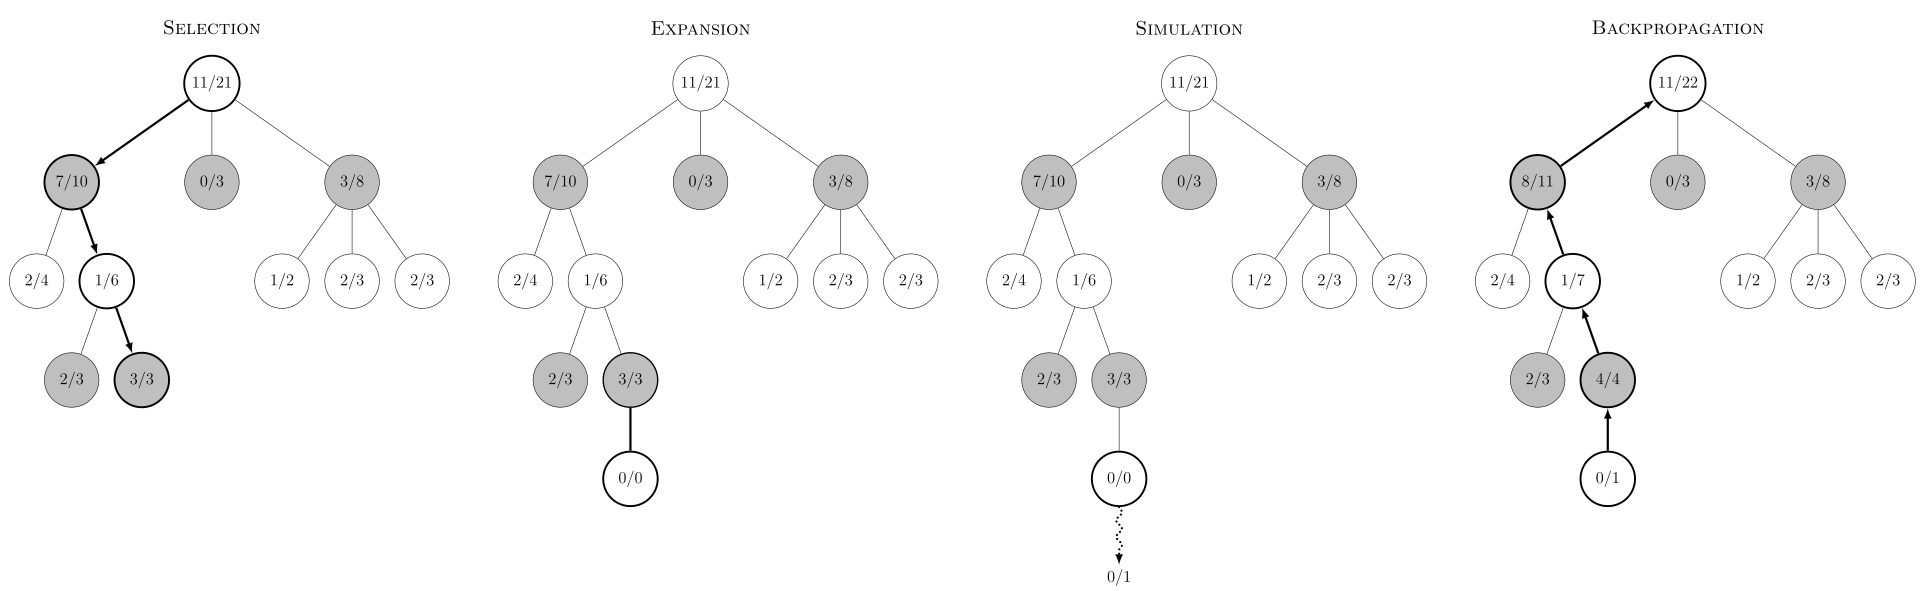
\includegraphics[scale=0.25]{MCTS-steps.png}
\caption{The $4$ phases in an MCTS iteration. Every node contains the number of visits and the accumulated value}
\end{figure}

A great benefit of MCTS is that the values of intermediate states do not have to be evaluated, as for depth-limited minimax search, which greatly reduces the amount of domain knowledge required. Only the value of the terminal state at the end of each simulation is required.\\
The {\tt python} code in appendix \ref{app:mcts} describes a fully-functional MCTS algorithm to find an optimal move for problem $P$.



% ######################################################################"
\section{Particle Filter}
\emph{Particle filters}, or sequential Monte Carlo methods, are a set of Monte Carlo algorithms used to solve filtering problems arising in signal processing and Bayesian statistical inference. The filtering problem consists of estimating the internal states in dynamical systems when partial observations are made and random perturbations are present in the sensors as well as in the dynamical system. The objective is to compute the posterior distributions of the states of a Markov process, given the noisy and partial observations.\\
More formally, a particle filter is a way to represent a probability distribution as a collection of samples, while this distribution is subject to a dynamic process $T(x, u, x') = p(x' | u, x)$. The basic idea is to approximate the posterior of a set of samples $\{x_t^{[i]}\}$. Each $x_t^{[i]}$ is a concrete sample of index $i$, where $i$ ranges from $1$ to $M$, the size of the article filter.\\
The basic version of the algorithm goes as follows:
\begin{itemize}
    \item \textbf{Initialization:} At time $t=0$, draw $M$ particles according to $p(x_0)$. Call this set of particles $X_0$.
    \item \textbf{Recursion:} 
    \begin{enumerate}
        \item At time $t>0$, generate a particle $x_t^{[i]}$ for each particle $x_t^{[i-1]} \in X_{t-1}$ by drawing from the actual model $p(x_t | u_t, x_{t-1}^{[i]})$. Call the resulting set $\bar X_t$.
        \item Subsequently, draw $M$ particles from $\bar X_t$, so that each $x_t^{[i]} \in \bar X_{t}$ is drawn (with replacement) with a probability proportional to $p(z_t | x_t^{[i]})$. Call the resulting set of particles $X_t$.
    \end{enumerate}
\end{itemize}

\begin{comment}
\begin{figure}[h]
	\centering
	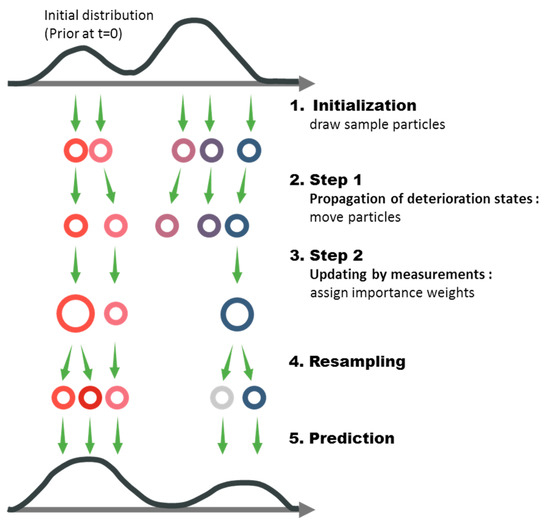
\includegraphics[scale=1]{particle-filter.jpg}
	\caption{The $4$ phases in an MCTS iteration. Every node contains the number of visits and the accumulated value}
\end{figure}
\end{comment}

\begin{thebibliography}{9}
	\bibitem{silver2010}
	Silver, David, and Joel Veness. "Monte-Carlo planning in large POMDPs." Advances in neural information processing systems 23 (2010).
	
	\bibitem{kocsis2006}
	L. Kocsis and C. Szepesvari. Bandit based Monte-Carlo planning. In 15th European
	Conference on Machine Learning, pages 282–293, (2006).
	
\end{thebibliography}

\newpage
\appendix
\section{MCTS Implementation}
\label{app:mcts}

\begin{minted}{python}
    class MCTS:
        def __init__(self, problem, T=1, c=2):
            """T = time to explore before returning anwser
               c = exploration factor"""
            self.problem = problem
            self.T = T
            self.c = c
    
            self.visits = {}
            self.values = {}
        
        def run(self, root):
            self.visits[root], self.values[root] = 0, 0
            self.tree = {}
            start_time = time.time()
            while time.time() - start_time < self.T:
                leaf_node, trace = self.select(root)
                if self.problem.terminal(leaf_node):
                    value = self.problem.value(leaf_node)
                else:
                    children = self.expand(leaf_node)
                    next_child, _ = children[0] # always start with first child from new children
                    value = self.rollout(next_child)
                self.backprop(value, trace)
            root_vals = [(self.values[child]/self.visits[child], action)
                        for child, action in self.tree[root]]
            _, action = sorted(root_vals)[-1] # pick action that leads
                                              # to child with highest value/visit
            return action
        
        def select(self, node):
            trace = [node]
            while node in self.tree: # if not in tree -> expand (i.e. is leaf node)
                N = self.visits[node]
                uct = []
                for child, _ in self.tree[node]:
                    if child not in self.visits or self.visits[child] == 0:
                        uct.append((np.infty, child))
                    else:
                        uct.append((self.c * np.sqrt(np.log(N)/self.visits[child]), child))
                v, node = max(uct)
                trace.append(node)
            return node, trace
    
        def expand(self, node) -> None:
            children = [(self.problem.step(node, action)[0], action)
                        for action in self.problem.all_actions()]
            self.tree[node] = children
            for child, _ in children:
                self.visits[child], self.values[child] = 0, 0
            return children
    
        def _rollout_policy(self, state):
            return random.choice(self.problem.all_actions())
    
        def rollout(self, state) -> float:
            terminal = self.problem.terminal(state)
            if terminal:
                self.problem.value(state)
            while not terminal:
                action = self._rollout_policy(state)
                state, terminal = self.problem.step(state, action)
            return self.problem.value(state)
    
        def backprop(self, value, trace) -> None:
            for node in trace:
                self.visits[node] += 1
                self.values[node] += value
                
    
    if __name__ == '__main__':
        problem = Problem()
        mcts = MCTS(problem)
        state = problem.init_state()
        while not problem.terminal(state):
            action = mcts.run(state)
            state, _ = game.move(state, move)
    
    \end{minted}





\end{document}